\chapter*{Tutorial 3}

Create a new struct to send and receive from Server and Client.

\section{Client}
\begin{verbatim}

create a new file (process_X.cfg) for the configuration of the process

process(
	name = Process_X
	SHM = SHM_X
	Subscriber = cmd_vel
	Publisher = odom_1
 	Node2RTAI  = posWheels
	RTAI2Node  = posWheels
	IP_RTAI  = 140.78.133.43
	PORT_RTAI  = 1101
)

In the file "AaronMR_Robotic_Stack/Drivers/CB_TCP_RTAI/include/TCP_RTAI/comStruct.h" create a new struct:

  struct posWheels_t
  {
    Point pos_W[4];
  };


In the file "AaronMR_Robotic_Stack/Drivers/CB_TCP_RTAI/include/TCP_RTAI/structType_C.hpp", create a new subclass:

class struct_posWheels : public structType {

public:
    posWheels();
    int serialize(char* data2s);
    int Unserialize(char* data2us);
    void* set_Publisher(char* name);
    void* set_Subscriber(char* name);

    ros::NodeHandle n;
    ros::Publisher posWheels_pub;
    ros::Subscriber posWheels_sub;

    // struct to send and receive
    posWheels_t data2send;
    posWheels_t data2recv;

    geometry_msgs::Point point_msg;
    void cmdCallback(const geometry_msgs::Point &data_);
    bool haveSubscriber;
    bool havePublisher;
    pthread_mutex_t mutex;
    bool canRecv_t;
    bool canSend_t;
    bool canSend();
    bool canRecv();
    int spinOnce();
};


create a new file for the new class, "struct_posWheels.cpp" with the content:

#include "pack2.hpp"
#include "structType_C.hpp"

struct_posWheels::struct_posWheels()
{

}

void struct_posWheels::cmdCallback(const geometry_msgs::Point &data_)
{

}

void* struct_posWheels::set_Subscriber(char* name)
{

}

void* struct_posWheels::set_Publisher(char* name)
{

}

bool struct_posWheels::canSend()
{

}

bool struct_posWheels::canRecv()
{

}

int struct_posWheels::spinOnce()
{

}

int struct_posWheels::serialize(char* data2s)
{

}

int struct_posWheels::Unserialize(char* data2us)
{

}


In the constructor:

struct_posWheels::struct_posWheels()
{

    haveSubscriber  = false;
    havePublisher   = false;
    canRecv_t       = true;
    canSend_t       = true;
    mutex           = PTHREAD_MUTEX_INITIALIZER;

}


Configure the functions to serialize and unserialize:

int struct_posWheels::serialize(char* data2s)
{
   
    unsigned char buf[1024];
    unsigned char magic;
    unsigned int packetsize;
    unsigned int ps2;

    posWheels_t aux;

    aux.pos_W[0].x = 0.0;
    aux.pos_W[0].y = 0.0;
    aux.pos_W[0].z = 0.0;

    aux.pos_W[1].x = 0.0;
    aux.pos_W[1].y = 0.0;
    aux.pos_W[1].z = 0.0;

    aux.pos_W[2].x = 0.0;
    aux.pos_W[2].y = 0.0;
    aux.pos_W[2].z = 0.0;

    aux.pos_W[3].x = 0.0;
    aux.pos_W[3].y = 0.0;
    aux.pos_W[3].z = 0.0;

    packetsize = pack(buf, "CHdddddddddddd",  'A',
					      0,
                                              aux.pos_W[0].x,
                                              aux.pos_W[0].y,
                                              aux.pos_W[0].z,
                                              aux.pos_W[1].x,
                                              aux.pos_W[1].y,
                                              aux.pos_W[1].z,
                                              aux.pos_W[2].x,
                                              aux.pos_W[2].y,
                                              aux.pos_W[2].z,
                                              aux.pos_W[3].x,
                                              aux.pos_W[3].y,
                                              aux.pos_W[3].z);

    packi16(buf+1, packetsize); // store packet size in packet for kicks
    memcpy((unsigned char*)data2s, buf, packetsize);

    return 0;
}

int struct_posWheels::Unserialize(char* data2us)
{

    unsigned char buf[1024];
    unsigned char magic;
    unsigned int ps2;

    memcpy(buf, data2us, 1024);

    posWheels_t aux;

    aux.pos_W[0].x = 0.0;
    aux.pos_W[0].y = 0.0;
    aux.pos_W[0].z = 0.0;

    aux.pos_W[1].x = 0.0;
    aux.pos_W[1].y = 0.0;
    aux.pos_W[1].z = 0.0;

    aux.pos_W[2].x = 0.0;
    aux.pos_W[2].y = 0.0;
    aux.pos_W[2].z = 0.0;

    aux.pos_W[3].x = 0.0;
    aux.pos_W[3].y = 0.0;
    aux.pos_W[3].z = 0.0;

    unpack((unsigned char*)buf, "CHdddddddddddd",&magic,
                                                &ps2,
                                                &aux.pos_W[0].x,
                                                &aux.pos_W[0].y,
                                                &aux.pos_W[0].z,
                                                &aux.pos_W[1].x,
                                                &aux.pos_W[1].y,
                                                &aux.pos_W[1].z,
                                                &aux.pos_W[2].x,
                                                &aux.pos_W[2].y,
                                                &aux.pos_W[2].z,
                                                &aux.pos_W[3].x,
                                                &aux.pos_W[3].y,
                                                &aux.pos_W[3].z);


    return 0;
}


In the file "AaronMR_C.cpp", add the next lines:

// Configure type of struct to send
...
else if(configuration[0].Node2RTAI.compare("posWheels") == 0)
{
  structToSend = new struct_posWheels;
}

// configure type of struct to receive
...
else if(configuration[0].RTAI2Node.compare("posWheels") == 0)
{
  structToRecv = new struct_posWheels;
}

\end{verbatim}

\section{Server}

\begin{verbatim}

Add a new configuration in the file "ServerFile.cfg" for the configuration of the new process

process(
	name = Process_X
	SHM = SHM_X
	Subscriber = cmd_vel
	Publisher = odom_1
 	Node2RTAI  = posWheels
	RTAI2Node  = posWheels
	IP_RTAI  = 140.78.133.43
	PORT_RTAI  = 1101
)

In the file "comStruct.h" add the new struct_posWheels

struct posWheels_t
{
  Point pos_W[4];
}

Create a new class in the structType_S.cpp

    class struct_posWheels : public structType {
    public:
      struct_posWheels();
      char* serialize(char* data2s);
      char* Unserialize(char* data2us);
      void storeData(Joy *joy);
      Joy auxJoy1;

      void iniSHM(int shm_in, int shm_out, char* SHM_name);

      Pose auxPose1;
      int sizeof_Joy;
      bool haveSubscriber;
      bool havePublisher;

      struct posWheels_t *dataIN;
      struct posWheels_t *dataOUT;

    };

Create a new file for the new class, "struct_posWheels.cpp" with the content

#include "AaronMR_S.hpp"
#include "pack2.hpp"
#include <rtai_shm.h>

struct_posWheels::struct_posWheels()
{
   auxSerialize.pos_W[0].x = 0.0;
   auxSerialize.pos_W[0].y = 0.0;
   auxSerialize.pos_W[0].z = 0.0;

   auxSerialize.pos_W[1].x = 0.0;
   auxSerialize.pos_W[1].y = 0.0;
   auxSerialize.pos_W[1].z = 0.0;

   auxSerialize.pos_W[2].x = 0.0;
   auxSerialize.pos_W[2].y = 0.0;
   auxSerialize.pos_W[2].z = 0.0;

   auxSerialize.pos_W[3].x = 0.0;
   auxSerialize.pos_W[3].y = 0.0;
   auxSerialize.pos_W[3].z = 0.0;

   auxUnSerialize.pos_W[0].x = 0.0;
   auxUnSerialize.pos_W[0].y = 0.0;
   auxUnSerialize.pos_W[0].z = 0.0;

   auxUnSerialize.pos_W[1].x = 0.0;
   auxUnSerialize.pos_W[1].y = 0.0;
   auxUnSerialize.pos_W[1].z = 0.0;

   auxUnSerialize.pos_W[2].x = 0.0;
   auxUnSerialize.pos_W[2].y = 0.0;
   auxUnSerialize.pos_W[2].z = 0.0;

   auxUnSerialize.pos_W[3].x = 0.0;
   auxUnSerialize.pos_W[3].y = 0.0;
   auxUnSerialize.pos_W[3].z = 0.0;

}

void struct_posWheels::iniSHM(int shm_in, int shm_out, char* SHM_name)
{
   if (shm_in == 1)
   {
       dataIN = (posWheels_t*)rtai_malloc (nam2num(SHM_name), sizeof(struct posWheels_t)) ;

       dataIN->pos_W[0].x = 0.1;
       dataIN->pos_W[0].y = 0.2;
       dataIN->pos_W[0].z = 0.3;

       dataIN->pos_W[1].x = 0.4;
       dataIN->pos_W[1].y = 0.5;
       dataIN->pos_W[1].z = 0.6;

       dataIN->pos_W[2].x = 0.7;
       dataIN->pos_W[2].y = 0.8;
       dataIN->pos_W[2].z = 0.9;

       dataIN->pos_W[3].x = 0.10;
       dataIN->pos_W[3].y = 0.11;
       dataIN->pos_W[3].z = 0.12;
   }

   if (shm_out == 1)
   {
       dataOUT = (posWheels_t*)rtai_malloc (nam2num(SHM_name), sizeof(struct posWheels_t)) ;

       dataOUT->pos_W[0].x = 1.0;
       dataOUT->pos_W[0].y = 2.0;
       dataOUT->pos_W[0].z = 3.0;

       dataOUT->pos_W[1].x = 4.0;
       dataOUT->pos_W[1].y = 5.0;
       dataOUT->pos_W[1].z = 6.0;

       dataOUT->pos_W[2].x = 7.0;
       dataOUT->pos_W[2].y = 8.0;
       dataOUT->pos_W[2].z = 9.0;

       dataOUT->pos_W[3].x = 10.0;
       dataOUT->pos_W[3].y = 11.0;
       dataOUT->pos_W[3].z = 12.0;
   }
}

char *struct_posWheels::serialize(char* buf3)
{
    unsigned char buf[1024];
    unsigned char magic;
    unsigned int packetsize, ps2;

   auxSerialize.pos_W[0].x = dataOUT->pos_W[0].x;
   auxSerialize.pos_W[0].y = dataOUT->pos_W[0].y;
   auxSerialize.pos_W[0].z = dataOUT->pos_W[0].z;

   auxSerialize.pos_W[1].x = dataOUT->pos_W[1].x;
   auxSerialize.pos_W[1].y = dataOUT->pos_W[1].y;
   auxSerialize.pos_W[1].z = dataOUT->pos_W[1].z;

   auxSerialize.pos_W[2].x = dataOUT->pos_W[2].x;
   auxSerialize.pos_W[2].y = dataOUT->pos_W[2].y;
   auxSerialize.pos_W[2].z = dataOUT->pos_W[2].z;

   auxSerialize.pos_W[3].x = dataOUT->pos_W[3].x;
   auxSerialize.pos_W[3].y = dataOUT->pos_W[3].y;
   auxSerialize.pos_W[3].z = dataOUT->pos_W[3].z;

   packetsize = pack(buf, "CHdddddddddddd", 'A',
                                       0,
                                       auxSerialize.pos_W[0].x,
                                       auxSerialize.pos_W[0].y,
                                       auxSerialize.pos_W[0].z,
                                       auxSerialize.pos_W[1].x,
                                       auxSerialize.pos_W[1].y,
                                       auxSerialize.pos_W[1].z,
                                       auxSerialize.pos_W[2].x,
                                       auxSerialize.pos_W[2].y,
                                       auxSerialize.pos_W[2].z,
                                       auxSerialize.pos_W[3].x,
                                       auxSerialize.pos_W[3].y,
                                       auxSerialize.pos_W[3].z
                                       );

   packi16(buf+1, packetsize); // store packet size in packet for kicks

   memcpy((unsigned char*)buf3, buf, packetsize);

    unpack((unsigned char*)buf3, "CHdddddddddddd",
                                           &magic,
                                           &ps2,
                                           &auxSerialize.pos_W[0].x,
                                           &auxSerialize.pos_W[0].y,
                                           &auxSerialize.pos_W[0].z,
                                           &auxSerialize.pos_W[1].x,
                                           &auxSerialize.pos_W[1].y,
                                           &auxSerialize.pos_W[1].z,
                                           &auxSerialize.pos_W[2].x,
                                           &auxSerialize.pos_W[2].y,
                                           &auxSerialize.pos_W[2].z,
                                           &auxSerialize.pos_W[3].x,
                                           &auxSerialize.pos_W[3].y,
                                           &auxSerialize.pos_W[3].z
                                           );

    printf("posWheels - send: '%c' %hhu %f %f %f %f %f %f %f %f %f %f %f %f\n",
                                           magic,
                                           ps2,
                                           auxSerialize.pos_W[0].x,
                                           auxSerialize.pos_W[0].y,
                                           auxSerialize.pos_W[0].z,
                                           auxSerialize.pos_W[1].x,
                                           auxSerialize.pos_W[1].y,
                                           auxSerialize.pos_W[1].z,
                                           auxSerialize.pos_W[2].x,
                                           auxSerialize.pos_W[2].y,
                                           auxSerialize.pos_W[2].z,
                                           auxSerialize.pos_W[3].x,
                                           auxSerialize.pos_W[3].y,
                                           auxSerialize.pos_W[3].z
                                           );

}

char *struct_posWheels::Unserialize(char* buf3)
{

   unsigned char buf[1024];
    unsigned char magic;
    unsigned int ps2;

   memcpy(buf, buf3, 1024);

    unpack((unsigned char*)buf, "CHdddddddddddd",
                                           &magic,
                                           &ps2,
                                           &auxUnSerialize.pos_W[0].x,
                                           &auxUnSerialize.pos_W[0].y,
                                           &auxUnSerialize.pos_W[0].z,
                                           &auxUnSerialize.pos_W[1].x,
                                           &auxUnSerialize.pos_W[1].y,
                                           &auxUnSerialize.pos_W[1].z,
                                           &auxUnSerialize.pos_W[2].x,
                                           &auxUnSerialize.pos_W[2].y,
                                           &auxUnSerialize.pos_W[2].z,
                                           &auxUnSerialize.pos_W[3].x,
                                           &auxUnSerialize.pos_W[3].y,
                                           &auxUnSerialize.pos_W[3].z
                                           );

    printf("posWheels - recv: '%c' %hhu %f %f %f %f %f %f %f %f %f %f %f %f\n",
                                           magic,
                                           ps2,
                                           auxUnSerialize.pos_W[0].x,
                                           auxUnSerialize.pos_W[0].y,
                                           auxUnSerialize.pos_W[0].z,
                                           auxUnSerialize.pos_W[1].x,
                                           auxUnSerialize.pos_W[1].y,
                                           auxUnSerialize.pos_W[1].z,
                                           auxUnSerialize.pos_W[2].x,
                                           auxUnSerialize.pos_W[2].y,
                                           auxUnSerialize.pos_W[2].z,
                                           auxUnSerialize.pos_W[3].x,
                                           auxUnSerialize.pos_W[3].y,
                                           auxUnSerialize.pos_W[3].z
                                           );

   dataIN->pos_W[0].x = auxUnSerialize.pos_W[0].x;
   dataIN->pos_W[0].y = auxUnSerialize.pos_W[0].y;
   dataIN->pos_W[0].z = auxUnSerialize.pos_W[0].z;

   dataIN->pos_W[1].x = auxUnSerialize.pos_W[1].x;
   dataIN->pos_W[1].y = auxUnSerialize.pos_W[1].y;
   dataIN->pos_W[1].z = auxUnSerialize.pos_W[1].z;

   dataIN->pos_W[2].x = auxUnSerialize.pos_W[2].x;
   dataIN->pos_W[2].y = auxUnSerialize.pos_W[2].y;
   dataIN->pos_W[2].z = auxUnSerialize.pos_W[2].z;

   dataIN->pos_W[3].x = auxUnSerialize.pos_W[3].x;
   dataIN->pos_W[3].y = auxUnSerialize.pos_W[3].y;
   dataIN->pos_W[3].z = auxUnSerialize.pos_W[3].z;

   return NULL;
}


Add the next lines in the "AaronMR_S.cpp" file

// configuration send structure
  ...
  ...
}else if(processThread_2.Node2RTAI.compare("posWheels") == 0){
       //Node2RTAI = 6;
       structToRecv = new struct_posWheels;
       structToRecv->iniSHM(1, 0, (char*)processThread_2.SHM_IN.data());
}

...
...
// configuration recv structure
  ...
  ...
}else if(processThread_2.RTAI2Node.compare("posWheels") == 0){
       //RTAI2Node = 6;
       structToSend = new struct_posWheels;
       structToSend->iniSHM(0,1, (char*)processThread_2.SHM_OUT.data());
}

\end{verbatim}


%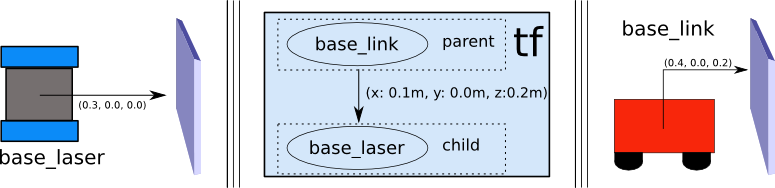
\includegraphics[width=0.5\textwidth,angle=0]{tutorials/tutorial_2/img/tf_robot.png}